\graphicspath{ {img/Sarnoff/} }
\chapter{An MDP Framework for Centralized Dynamic Spectrum Leasing}\label{Sarnoff_chap}
\section{Introduction}
In the next two chapters we propose two automated spectrum trading mechanisms, suitable for different scenarios. The one described in this chapter is appropiate for situations of low spectrum usage by PUs. In such scenario, the spectrum owner may be willing to obtain some benefit from its unused resource by selling it to SUs. Nevertheless, it still has to meet the demands of the PUs (to some extent), assuring that the blocking probability for the PUs remains under a desired threshold. We show how to compute a policy that balances those two objectives by means of an MDP and a constrained-MDP formulations. 

\subsection{Motivation}
In situations of low spectrum usage, a licensed operator may decide to sell spectrum opportunities to SUs in the \textit{secondary spectrum market} to obtain extra-revenue from its resources. A regulator may encourage this behavior, for example, by setting a fee proportional to the amount of spectrum held. \cite{AdvisorsonScience}.  

The operator does not know the future demands from its users in advance (apart from a statistical characterization). What would happen if, at any given moment, all of its spectrum is in use and a new PU arrives to the system? As the licensed operator, it could reclaim the spectrum it leased to SUs if needed, but the process is not inmediate and the incurred delay could result in, for example, a PU missed call. We refer to the probability of such event as the \emph{blocking probability}. In addition, reclaiming its spectrum may not be a convenient solution for the operator (\textit{e.g.} because it may require a compensation to the SU). 

Therefore, a licensed operator should carefully balance the revenue obtained from allowing the SUs to access its spectrum, with the blocking probability of the PUs. In order to do this in real-time, a protocol is required to support negotiations on access price, channel holding time, \textit{etc}., between the spectrum owner and the SUs. In this work, we consider a centralized bid-auction model, in which SUs bid for the spectrum of a single spectrum owner. We consider a continuous bid process, in which each incoming SU makes its bid upon arrival. Because of the real-time constraint, the operator only knows one bid at a time, and has to make its decision for each incoming SU, before knowing future bids.
We explore the use of MDP and CMDP formulations to balance benefit and grade of service for PUs. The main advantages of this approach is that it assures operating at global optimum and reduces the computational effort at SUs.

\subsection{Related Work}\label{sec:Application}

Centralized dynamic spectrum trading has been addressed in previous works. In the proposal by Yu \textit{et. al.} \cite{ref:Yu2007}, the spectrum broker controls the access of SUs based on a threshold rule computed by means of an MDP formulation with the objective of minimizing the blocking probability of secondary users. In order to cope with the non-stationarity of traffic conditions, the authors propose a finite horizon MDP instead of an infinite horizon one. The drawback is that the policy cannot be computed off-line, imposing a high computational overhead on the system.
Tang \textit{et. al.} study in \cite{ref:Tang2009_per} several admission control schemes at a centralized spectrum manager. The objective is to meet the traffic demands of SUs, increasing spectrum utilization efficiency while assuring a grade of service in terms of blocking probability to primary users. Among the schemes analyzed, the best performing one is based on a constrained Markov decision process (CMDP).

When the problem is distributed, dynamic game theory is used instead of MDP.
In \cite{ref:Niyato}, spectrum trading from PUs to SUs is modeled as a non-cooperative dynamic game, using a Markov chain to describe groups of SUs buying opportunities from PUs. Given its distributed implementation, the main goal of this approach is finding the system's equilibrium. The objective in \cite{ref:eBay} and \cite{ref:Jia} is maximizing the profit of PUs, with especial interest in assuring bidding truthfulness. Wang \textit{et. al.} present in \cite{ref:Wang} a bandwidth auction mechanism between an PU and multiple SUs, where the objective is to maximize the SU's payoff and reach Nash equilibrium in a competitive and distributed manner, while the PU sets a minimum remaining bandwidth for its own use as a constraint. 

\subsection{Our contribution}

This chapter addresses the design of centralized DSA MAC protocols for real-time dynamic spectrum auction. We explore the possibilities of a formal design based on a Markov decision process (MDP) formulation and propose, in Section \ref{Sarnoff_sec_model}, a design framework to balance the grade-of-service (given by the blocking probability for PUs) and the expected economic revenue provided by the SUs' accepted bids. This trade-off can be managed in two ways. One consists of computing a single objective value given by a combination of the blocking probability and the expected revenue. The weights assigned to each objective determine the point in the Pareto front where the obtained policy lies. The other approach, which is presented in Section \ref{sec:Constrained MDP}, consists of solving for one of the objectives and setting constraints on the remaining ones.
This strategy results in a constrained MDP formulation (CMDP) and the policies obtained are not necessarily deterministic.

\section{System model}\label{Sarnoff_sec_model}

The model includes a spectrum bidding procedure in which SUs send their bid offers, within a finite countable set of prices (for mathematical tractability), for the use of a channel. Each bid offer consists of the price that the SU is willing to pay for each minute of channel holding time. Taking into account the trade-off between the blocking probability of PUs and the expected benefit obtained from spectrum rental, SUs can be accepted or rejected. Accepted SUs are given access to the band and they are charged for it the price they selected. PUs are always accepted if the there are available channels.
%As explained in the Sarnoff_sec_intro, public administrations assign the spectrum bands to wireless operators by a license scheme. Generally, operators gain spectrum licenses by bidding for them in public auction processes. We refer to this spectrum assignment framework as \textit{primary market}. The increasing demand of spectrum and the existence of spectrum holes have revealed the inefficiency of this mechanism. One practical and economically feasible way to solve this inefficiency is to allow spectrum owners to sell their spectrum opportunities in a \textit{secondary market}. In contrast to the primary market, the secondary operates in real-time.
%SUs, that may be operators without a spectrum license, submit their bids for spectrum opportunities to the spectrum owner, who determines the winner or winners by giving them access to the band and charging them the bidding price.

Incoming traffic is characterized by a classic Poisson model. PUs arrive with a rate of $\lambda_{L}$ arrivals per unit of time. The arrival rate for SUs is denoted by $\lambda_{U}$. The licensed spectrum managed by the central controller is assumed to be divided into channels (or bands) with equal bandwidth. Each user occupies a single channel. The average holding times for PUs and SUs are given by $1/\mu_{L}$ and $1/\mu_{U}$ respectively, where $\mu_{L}$ and $\mu_{U}$ denote the departure rate for each class. Because a Poisson traffic model is considered, both the inter-arrival time and the channel holding times are exponentially distributed random variables for both user classes. The model can be easily extended including more user classes, the probability that a user occupies two or more channels, and so on. Essentially the procedure is the same, but the Markov chain would comprise more states as more features are considered in the model. In this model, the state of the Markov chain is determined by the number of channels $k$ occupied by PUs, and the number of channels $s$ occupied by SUs. Because spectrum is a limited resource, there is a finite number $N$ of channels. Figure \ref{fig:Diagram2} depicts a diagram of the model and its parameters. Note that we can map all the possible combinations of $\left(k,s\right)$ for $0\leq k \leq N$, $0\leq s \leq N$ and $k+s \leq N$ into a single integer $i$ such that
\begin{equation}\label{states}
	  0 \leq i \leq \displaystyle\frac{N\left(N+1\right)}{2}+N+1.
\end{equation}
The number in the right hand side of previous equation is the total number of states that we will denote by $N_{T}$.

The bidding prices are classified into a finite set of values: $\mathbb{B}=\left\{b_{1},b_{2},\ldots b_{m}\right\}$ given in money charged per unit of time. Each price has a probability $p_{i}$ of being offered by an incoming user. Obviously $\sum^{m}_{i=1}p_{i}=1$. Figure \ref{fig:Diagram2} illustrates this model.

\begin{figure}[!t]
\centering
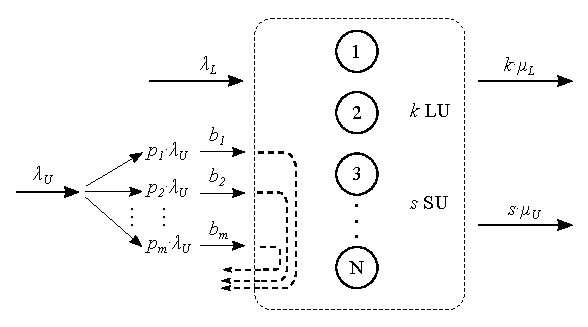
\includegraphics[scale=0.9]{diagram2.eps}
\caption[]{Diagram of the auction-based access model. SUs can offer up to $m$ different bid prices. Each  price is assigned a probability. The access policy decides upon each bid according to the price offered and the system's state.}
\label{fig:Diagram2}
\end{figure}

%This model is a continuous-time Markov chain. In this case, 
The objective of the MDP is to obtain the maximum economic profit with the minimum impact on PUs. In the framework of MDPs we have to define the actions and the costs of these actions.
%According to the objective, the expected cost is obtained as a linear combination of the blocking probability of the primary users and the income benefit from SUs. By adjusting the weighting factors we can compute a Pareto front for both elements. 
 Let $g(i,u)$ denote the instantaneous cost of taking action $u$ at state $i$. The control $u$ at each stage determines the admitted and rejected bidding prices. Logically, the control should be defined as a threshold, \textit{i.e.} when $u = i$ only bids equal or above $p_{i}$ are admitted. For notation convenience, the control $u = m+1$ indicates that no bid is accepted. The per-stage reward function $g(i,u)$ is given by the linear combination of the the blocking probability per unit of time, $g_{L}(i,u)$, and the expected benefit at stage $i$ when decision $u$ is made, $g_{U}(i,u)$. Therefore $g(i,u)$ =  $\alpha g_{L}(i,u)$ + $\beta g_{U}(i,u)$ where the scalars $\alpha$ and $\beta$ are weighting factors. Note that $\beta < 0$ since the objective is to minimize $g(i,u)$. By adjusting $\alpha$ and $\beta$ we can compute a Pareto front for both objectives.

The function $g_{L}(i,u)$, is given by the probability that the system cannot provide a channel to an incoming PU:
\begin{equation} \label{gLpriority}
	  g_{L}(i,u) =
	  \begin{cases}
		1,& \text{ if }i \equiv (k,s) \text{ and } k+s = N\\	 
		0,& \text{ otherwise} \\
 \end{cases}
\end{equation}
where the symbol ``$\equiv$'' denotes equivalence, \textit{i.e.} $i$ corresponds to a state $(k,s)$ such that $k+s = N$.

To determine $g_{L}(i,u)$, let $B_{i}$ denote the expected income when an SU whose bidding price is $b_{i}$ is accepted. Since the average channel holding time for PUs is $1/\mu_{U}$, then $B_{i} = b_{i}/\mu_{U}$.
Given a control $u$, $P\left(r | u\right)$ denotes the conditional probability that the bidding price of the next accepted SU is $b_{r}$, and is given by
\begin{equation}
	  P\left(r |u\right) =
	  \begin{cases}
		\displaystyle\frac{p_{r}}{\sum^{m}_{j = u}p_{j}}, & \text{ if }r \geq u\\	
		0, & \text{ otherwise } \\
 \end{cases}
\end{equation}
Let us define $\tilde{g}_{U}(i,u,j)$ as the average benefit associated to the transition from state $i$ to state $j$. Its expression is
\begin{equation}
	  \tilde{g}_{U}(i,u,j) =
	  \begin{cases}
		p_{U}\sum^{m}_{r = 1}B_{r}P\left(r | u\right), & \text{ if }j = i+1\\	
		0, & \text{ otherwise} \\
 \end{cases}
\end{equation}
where $p_{U} = \lambda_{U}/(\lambda_{U}+\lambda_{L})$ denotes the probability that the next arrival corresponds to an SU.
Therefore, the per-stage benefit $g_{U}(i,u)$ is given by
\begin{equation}\label{gUauction}
\begin{array}{lcl}
g_{U}(i,u) & = & \sum^{N_{T}}_{j = 1}\tilde{g}_{U}(i,u,j)p_{ij}(u)\\
					& = & p_{i,i+1}(u)p_{U}\sum^{N_{T}}_{j = 1}B_{r}P\left(r |u\right).
	\end{array}
\end{equation}

%The problem can be solved by solving equation (\ref{BellmanEq}) with the cost functions and transition probabilities corresponding to this model.
The objective is to find a policy minimizing the expected value of the combined cost, given by
\begin{equation}	 \lim_{K\rightarrow\infty}\frac{1}{E\left\{t_{K}\right\}}
E\left\{\int^{t_{K}}_{0}g\left(x(t),u(t)\right)\right\}
\end{equation}
where $t_{K}$ is the completion time of the $K$-th transition. The problem can be solved by formulating its auxiliary discrete-time average cost problem. Let $\gamma$ be a scalar greater than the transition rate out of any state of the chain, \textit{i.e.} $\gamma > v_{i}(u)$ for every $i$.
%, where $v_{i}(u)$ is the transition rate out of state $i$
We can compute the transition probabilities $\tilde{p}_{ij}(u)$ for the auxiliary discrete-time problem from the probabilities $p_{ij}(u)$ of the original problem as
\begin{equation}
	  \tilde{p}_{ij}(u) =
	  \begin{cases}
		\frac{v_{i}(u)}{\gamma}p_{ij}(u) &, \text{ if }i \neq j\\	
		1- \frac{v_{i}(u)}{\gamma}&, \text{ if }i = j \\
 \end{cases}
\end{equation}

%We can formulate the auxiliary discrete-time average cost problem for the model described. 
%The equation providing the optimum average cost $\lambda$ is
We can now formulate Bellman's equation (see \cite{ref:Bertsekas}) to obtain the optimum average cost $\lambda$
%It is known (see \cite{ref:Bertsekas}) that if the scalar $\lambda$ and the vector $\tilde{h}$ satisfy
\begin{equation}\label{BellmanEqAuction}
\tilde{h}\left(i\right) = \min_{u\in \left\{0,1\right\}}\biggl[\alpha g_{L}(i,u) + \beta g_{U}(i,u)v_{i}(u) -
 \lambda + \displaystyle\sum_{j=1}^{N_{T}}\tilde{p}_{ij}\bigl(u\bigr)\tilde{h}\left(j\right)\biggr]
\end{equation}
for $i =1,\ldots,n$. Multiplying $g_{U}(i,u)$ by $v_{i}(u)$ yields benefit per unit of time.
%then $\lambda$ and the vector $h$ with components $h(i) = \gamma\tilde{h}(i)$ solve the original problem. 
It can be anticipated that the structure of this problem, essentially a connection admission control problem, requires a threshold type solution in which upcoming SUs of each class will only be admitted into the system if the number of occupied channels is below certain threshold. There will be one threshold per bidding price. By properly adjusting the weighting factors $\alpha$ and $\beta$ we can compute a Pareto front allowing us to determine the maximum possible benefit for a given blocking objective for the PUs.
 
\section{Constrained MDP}\label{sec:Constrained MDP}
%So far, the approach to merge several objectives consisted on combining them into a single objective by means of a weighted sum and solving the problem as a conventional MDP. However, 
When several objectives concur in an MDP problem, another feasible approach is to optimize one of them subject to constraints on the other objectives. This strategy results in a CMDP formulation of the problem. Solving MDPs by iterative methods such as policy or value iteration allows us to find deterministic policies, \textit{i.e.} policies that associate each system's state $i \in S$ to a single control $u$.
% \in U(i)$, where $U(i)$ is a subset of $U$ containing the controls allowed in state $i$. 
However, these policies do not, in general, solve CMDP problems. Instead, the solution of a CMDP is a randomized policy, \textit{i.e.} it associates each state to a probability distribution defined over the elements in $U(i)$.

There are mainly two approaches to solve CMDPs, linear programming (LP) and Lagrangian relaxation of the Bellman's equation. This proposal follows the former one. Each feasible LP formulation relies on the use of the \textit{dual} variables $\phi\left(i,u\right)$, defined as the stationary probability that the system is in state $i$ and chooses action $u$ under a given randomized stationary policy. The problem addressed in this chapter results, under every stationary policy, in a truncated birth-death process, since PUs are always accepted. In consequence, every resulting Markov chain is \textit{irreducible}, in other words, it is recurrent and there are not transient states. Moreover, the state and action spaces are finite.
Under these circumstances, as shown in \cite{ref:Puterman}, every feasible solution of the LP problem corresponds to some randomized stationary policy. Therefore, if the constrained problem is feasible, then there exists an optimal randomized stationary policy.
%Under these circumstances, several results \cite{ref:Puterman} guarantee that every feasible solution of the LP problem corresponds to some randomized stationary policy resulting in the probabilities  and, what is even more important, if the constrained problem is feasible, then there exists an optimal randomized stationary policy.

The LP approach consists of expressing the objective and the constraints in terms of $\phi\left(i,u\right)$. Once the problem is discretized, the average cost is defined as
\begin{equation}\label{objective}
\lambda = \lim_{K\rightarrow\infty}\frac{1}{K}
E\left\{\sum^{K}_{k=0}g_{U}\left(x_{k},u_{k}\right)\right\}
\end{equation}
where $k$ denotes the decision epoch of the process.
The constraints are defined similarly to the main objective: each constraint imposes a bound on an average cost related to a different per-stage cost. In our case, it is given by
\begin{equation}\label{constraint}
c = \lim_{K\rightarrow\infty}\frac{1}{K}
E\left\{\sum^{K}_{k=0}g_{L}\left(x_{k},u_{k}\right)\right\} \leq \beta
\end{equation}
where $g_{L}\left(x(t),u(t)\right)$ is the real-valued function providing the per-stage cost associated to the constraint $\beta$. Therefore the average reward MDP with a single constraint is defined as the following minimization problem:
\begin{equation}
\min_{\mu} \lambda \text{ subject to } c \leq \beta
\end{equation}
Given the characteristics of the problem (finite state and action spaces and recurrent Markov chain under every policy), the limits in (\ref{objective}) and (\ref{constraint}) exist and are equal to
\begin{equation}
\lambda = \displaystyle\sum_{i\in S}\displaystyle\sum_{u\in U(i)}g_{U}\left(i,u\right)\phi\left(i,u\right)
\end{equation}
and
\begin{equation}
c = \displaystyle\sum_{i\in S}\displaystyle\sum_{u\in U(i)}g_{L}\left(i,u\right)\phi\left(i,u\right)
\end{equation}
respectively. In addition, the following conditions must be hold by the \textit{dual} variables:
\begin{equation}
\displaystyle\sum_{u\in U(j)}\phi\left(j,u\right) = \displaystyle\sum_{i\in S}\displaystyle\sum_{u\in U(i)}p_{ij}\left(u\right)\phi\left(i,u\right)
\end{equation}
for all $j \in S$, which is closely related to the balance equations of the Markov chain and
\begin{equation}
\displaystyle\sum_{i\in S}\displaystyle\sum_{u\in U(i)}\phi\left(i,u\right) = 1,
\end{equation}
which, together with $\phi\left(j,u\right) \geq 1$ for $i \in S$ and $u \in U(i)$ correspond to the definition of $\phi\left(i,u\right)$ as a limiting average state action frequency. In consequence, the LP for the CMDP has the following formulation:
\begin{equation}\label{CompleteCMDP}
\begin{array}{ll}
\underset{\phi}\min & \displaystyle\sum_{i\in S}\displaystyle\sum_{u\in U(i)}g_{U}\left(i,u\right)\phi\left(i,u\right) \\
\text{s.t.} & \displaystyle\sum_{i\in S}\displaystyle\sum_{u\in U(i)}g_{L}\left(i,u\right)\phi\left(i,u\right) \leq \beta\\
& \displaystyle\sum_{u\in U(j)}\phi\left(j,u\right) - \displaystyle\sum_{i\in S}\displaystyle\sum_{u\in U(i)}p_{ij}\left(u\right)\phi\left(i,u\right) = 0 \\
& \displaystyle\sum_{i\in S}\displaystyle\sum_{u\in U(i)}\phi\left(i,u\right) = 1\\
& \phi\left(j,u\right) \geq 1
\end{array}
\end{equation}
Assuming that the problem is feasible and $\phi^{*}$ is the optimal solution of the LP problem above, the stationary randomized optimal policy $\mu^{*}$ is generated by
\begin{equation}
q_{\mu^{*}\left(i\right)}\left(u\right)=\displaystyle\frac{\phi^{*}\left(i,u\right)}{\sum_{u' \in U(i)}\phi^{*}\left(i,u'\right)}
\end{equation}
for cases where the sum in the denominator is nonzero. Otherwise, the state is transitory and the control is irrelevant. Note that $q_{\mu^{*}\left(i\right)}\left(u\right)$ denotes the probability of choosing action $u$ at state $i$ under policy $\mu^{*}$.

\section{Numerical Results}\label{Sarnoff_sec_numerical}
We will consider three scenarios characterized by the asymmetry between the traffic intensity of PUs and SUs. In every scenario, the average holding time is equal for every user, independently of their type. Therefore the service rate $\mu_{L}$ =$\mu_{U}$ = 5. Assuming that the time unit is an hour, this results in an average holding time of 12 minutes per connection. The total traffic ($\lambda$ = $\lambda_{L}$ + $\lambda_{U}$) is 40 calls/h, which yields a total incoming traffic of 8 Erlangs. In a wireless cell covering 2.5 km$^{2}$ of urban area (cell radius equal to 400 m), with 2000 people per km$^{2}$ and a 10\% aggregate market penetration (PUs and SUs), the number of covered users is around 500, and the resulting traffic intensity is 0.016 Erlangs per user. The number of available channels is set to $N=10$, in order to evaluate the system in a relatively congested situation. With the assumed traffic intensity we can estimate the blocking probability of the system for the aggregate traffic by means of the well-known Erlang's B formula (see \cite{ref:Klei}):
\begin{equation}
E\left(n,\rho\right)=\displaystyle\frac{\frac{\rho^{n}}{n!}}{\sum_{j=0}^{j=n}\frac{\rho^{j}}{j!}}
\end{equation}
where $n$ is the number of channels and $\rho$ denotes the utilization factor. In our case $\rho$=$\lambda/\mu_{L}$ = $\lambda/\mu_{U}$. According to this formula, if the system accepted every incoming user, the total blocking probability would be $E\left(10,8\right)$=0.12. As we will see, this probability is an upper bound for the blocking probability of the PUs and a lower bound for the SUs.

The three scenarios are summarized in Table \ref{tab:table1}.

\begin{table}[h]
\centering
\begin{tabular}{lccc} \hline
 \textbf{Parameter} & \textbf{scenario 1} & \textbf{scenario 2} & \textbf{scenario 3}\\\hline
$\lambda_{L}$ (calls/h) & 30 & 20 & 10\\
$\lambda_{U}$ (calls/h) & 10 & 20 & 30\\
$\mu_{L}$=$\mu_{U}$ (calls/h) & 5 & 5 & 5\\
$N$ & 10 & 10 & 10\\\hline
\end{tabular}
\caption{Parameters setting for the three scenarios of the priority based access problem.}\label{tab:table1}
\centering
\end{table}

Additionally we define three classes of SUs, characterized by the price that they offer per minute of channel occupation. The bid offers per class are: class 1: 0.01 \$/m, class 2: 0.02 \$/m and class 3: 0.03 \$/m. We define the probability of an SU incoming call being of each class. The SU class probability distribution is: class 1 probability: 0.5, class 2 probability: 0.3 and class 3 probability: 0.2. We summarize SU class definition in Table \ref{tab:table2}.

\begin{table}[h]
\centering
\begin{tabular}{lccc} \hline
 \textbf{SU class} & \textbf{class 1} & \textbf{class 2} & \textbf{class 3}\\\hline
offered price (\$/m) & 0.01 & 0.02 & 0.03\\
probability & 0.5 & 0.3 & 0.2\\\hline
\end{tabular}
\caption{Classification of SUs in terms of their bid offers and their corresponding probabilities.}\label{tab:table2}
\centering
\end{table}
Note that both the offered prices and their probability distributions are static, \textit{i.e.} they do not change over time and are independent of the system occupation. It is not unrealistic taking into account typical tariff policies of wireless operators. In this environment the class structure and the probability distribution may be seen as types of contracts for SUs and market penetration of each type of contract respectively. However, for a more dynamical auction process, where bidders are able to change their bid offers adaptively, the model should be revised. One possibility would be to define one probability distribution for each state. More detailed modeling strategies would increase the complexity of the MDP solving algorithm or even make them intractable. This is a classic problem of MDPs, known as the \textit{curse of dimensionality} and is typically addressed by means of the heuristic approach of approximate dynamic programming.

\begin{figure}
\centering
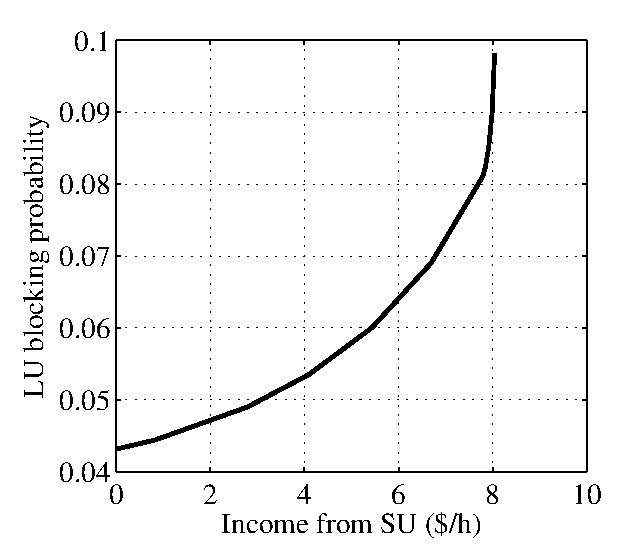
\includegraphics[scale=0.5]{MDPauction3010.eps}
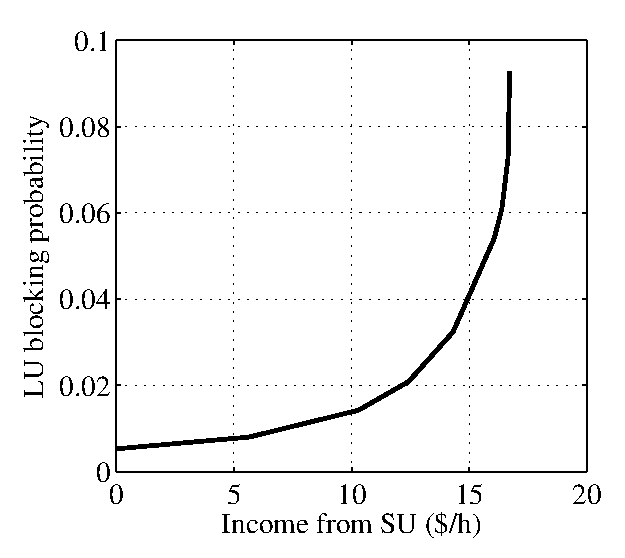
\includegraphics[scale=0.5]{MDPauction2020.eps} \\
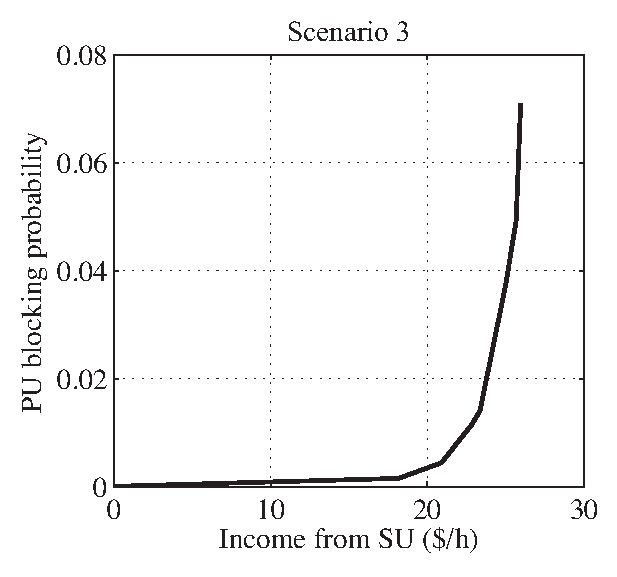
\includegraphics[scale=0.5]{MDPauction1030.eps}
\caption{Pareto fronts obtained for the auction-based access} \label{fig:MDPauction}
\end{figure}
% \begin{figure}[h]
% \centering
% \subfloat[scenario 1]{
% 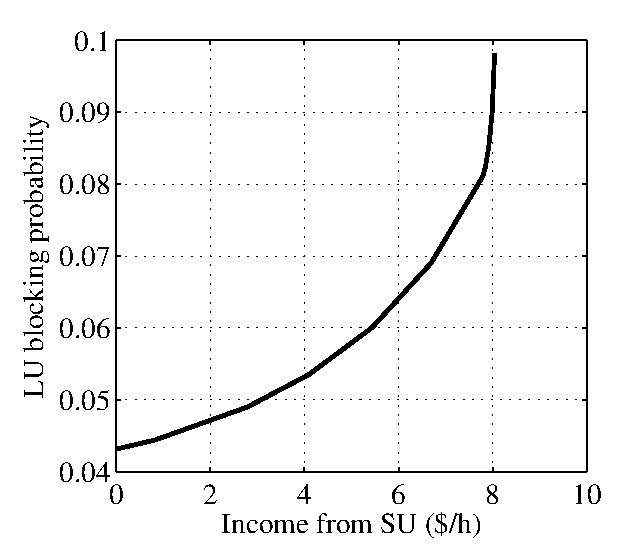
\includegraphics[scale=0.5]{MDPauction3010.eps}
% %\centerline{\psfig{figure=MDPauction3010.eps,width=3cm} }
% \label{fig:subfig1auction}
% }
% \subfloat[scenario 2]{
% 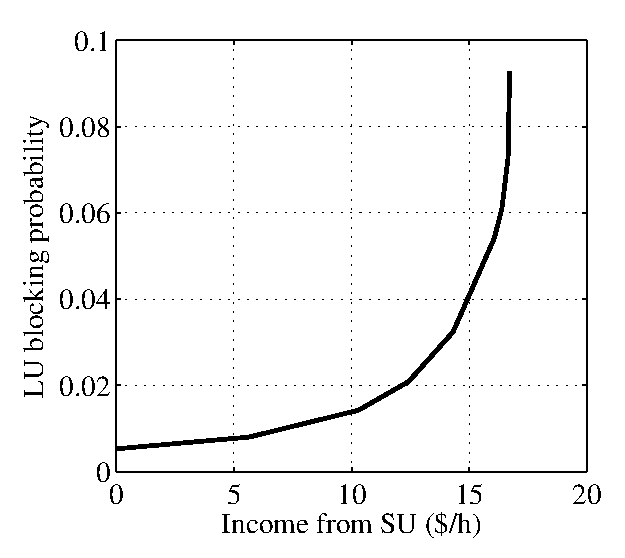
\includegraphics[scale=0.5]{MDPauction2020.eps}
% %\centerline{\psfig{figure=MDPauction2020.eps,width=3cm} }
% \label{fig:subfig2auction}
% } \\
% \subfloat[scenario 3]{
% 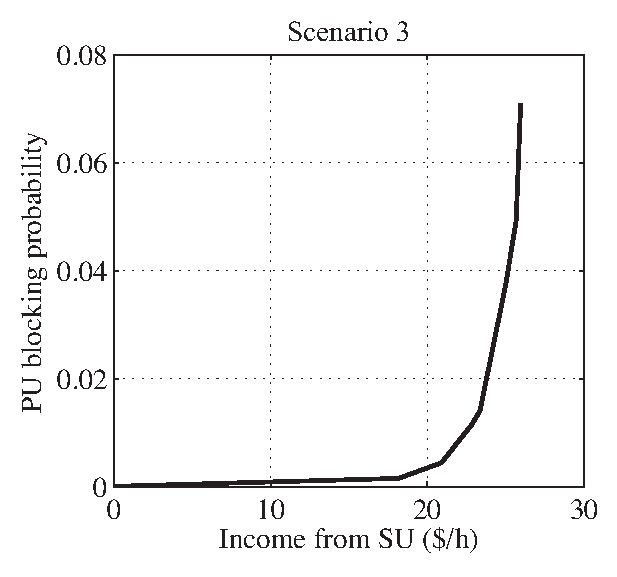
\includegraphics[scale=0.5]{MDPauction1030.eps}
% %\centerline{\psfig{figure=MDPauction1030.eps,width=3cm} }
% \label{fig:subfig3auction}
% }
% \caption[]{Pareto fronts obtained for the auction-based access}\label{fig:MDPauction}
% \end{figure}

Figure \ref{fig:MDPauction} shows the Pareto fronts for the auction-based system in the three scenarios. It can be observed that, for the same traffic intensity (the three scenarios receive 40 calls per unit of time) when the traffic share of the SUs is higher, the income obtained from SUs increases at the time that the blocking probability of the PUs diminishes. It is interesting to check that, especially in scenarios 2 and 3, a very small increment of PU blocking probability can multiply the benefit obtained from spectrum leasing by a factor of 2 or 3. On the other hand, these figures also indicate that once the income surpasses certain threshold, Pareto-optimal policies can only produce small increments of the income by dramatically rising PU blocking probability.

\begin{figure}[h]
\centering
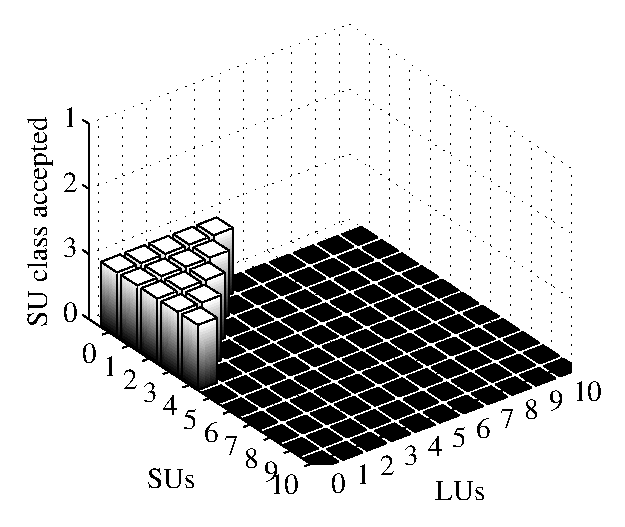
\includegraphics[scale=0.5]{Policy3010.eps}
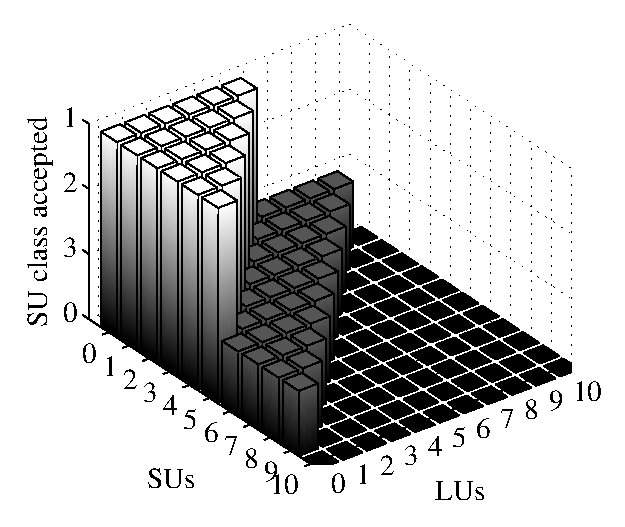
\includegraphics[scale=0.5]{Policy2020.eps}\\
\includegraphics[scale=0.5]{Policy1030.eps}
\caption[]{Graphical representation of policies attaining 0.04 PU blocking probability for the auction-based access}\label{fig:Policies}
\end{figure}

%A graphical representation of three policies of the first scenario can be observed in Fig. \ref{fig:Policies}. 
Fig. \ref{fig:Policies} shows the policies attaining a blocking probability for PUs of 0.04 for each scenario.
%The polices correspond to blocking probabilities for the PUs of 0.01, 0.02 and 0.03. 
The height of the bars corresponds to the lowest accepted class (prices) at each state. States where bars' height is $0$ correspond to states where all SUs are rejected, independently of their bids. As expected, Pareto-optimal policies are threshold type. As the traffic intensity of PUs reduces respect to that of the SUs, there are more states where SUs are admitted in the system, and lower prices are accepted, \textit{i.e.} the thresholds move toward smaller numbers. Interestingly, it is the total amount of occupied channels, and not the type of users occupying them, what determines the thresholds.
%This fact suggests that the analytical model can be simplified by notably reducing the size of state space. This would increase the feasibility of the procedure in higher dimensional problems, thus allowing the generalization of the model to \textit{e.g.} variable distributions of the bid offers. 

%In order to illustrate how policies change on the Pareto front, let us consider three different points of the Pareto front for scenario 2. These points correspond to the following blocking probabilities for PU: 0.01, 0.02 and 0.03.

\section{Conclusions}\label{Sarnoff_sec_conclusions}
In this chapter we propose an MDP framework for real-time auction-based spectrum leasing. The SUs are classified according to the price they are willing to pay for the use of the spectrum. The main issue of the problem addressed is that two contrary objectives coexist: to reduce blocking probability for PUs and to increase the income received from spectrum leasing. For these type of problems there does not exist an \textit{optimal} policy, but a set of \textit{Pareto optimal} policies. 

We have shown how to compute policies at the Pareto front by weighting the objectives in an MDP problem or by reformulating the problem as a constrained MDP. 
Numerical solutions of the proposed equations show the influence of the traffic share on system's performance and on the structure of Pareto-optimal policies. 



